\begin{figure}[p]
  \centering
  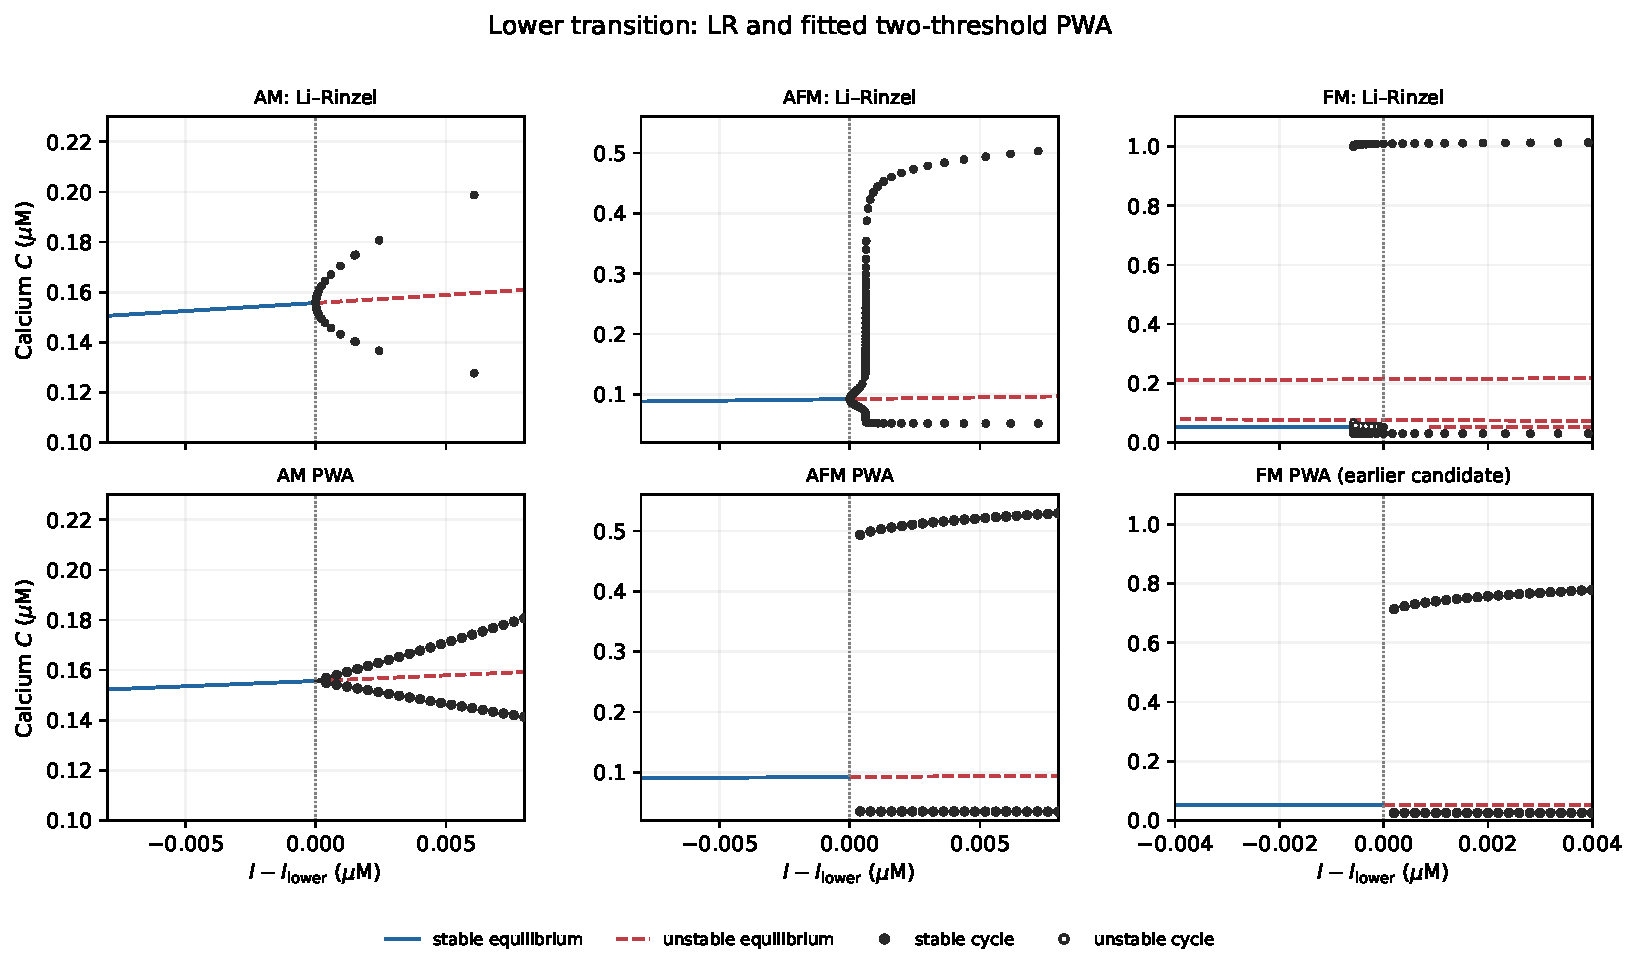
\includegraphics[width=\linewidth]{figures/figure5_lower_onset.pdf}
  \caption{Lower equilibrium transition and nearby cycle extrema in Li--Rinzel (top) and mixed-coordinate two-threshold PWA models (bottom) for AM, AFM, and FM. Each column uses the same input and calcium scales for the reference and PWA panels. The reference $I_{\rm lower}$ is the lower LR spectral Hopf candidate and the prescribed PWA equilibrium threshold crossing. Solid blue and dashed red curves represent stable and unstable equilibria, respectively; saddle equilibria are included among the latter. Filled and open markers denote stable and unstable cycle extrema. Reference cycles come from collocation continuation and local Hopf seeds, subject to independent finite-time integration checks. PWA cycles come from finite forward trajectories and a finite multistart search using boundary matching; the AM local curve is reconstructed from a one-threshold match and affine scaling. These finite searches do not establish absence of other cycles. AFM/FM local HLB2 candidates previously found under an exactly imposed boundary equilibrium lie below the resolution of these horizontal scales and are not drawn. The FM PWA is an earlier candidate from the free-hidden archive; the final frozen FM candidate was unavailable locally.}
  \label{fig:lower-onset}
\end{figure}
